As explained in the previous chapter, the Stratum Reference Implementation (SRI), is a full open-source, community based implementation of the Stratum V2 protocol specifications. The team who is building it started some years ago, and it's composed by independent developers majorly funded by individual grants. The project is supported by many companies involved into mining operations, such as Braiins, Foundry, Galaxy Digital. In addiction to them, there are engaged also entities like Bitmex, Human Rights Foundation, Spiral and the Summer of Bitcoin.\\
Nowadays, most of the implementation work has been done, but there are still some open discussions related to the protocol specifications, such as roles structure, noise encryption, job negotiation/declaration protocol.\\
However, as previously anticipated, Stratum V2 is a very flexible protocol, especially if compared to the current one used for pooled mining operations (Stratum V1). To fill the lack of flexibility of its predecessor, Stratum V2 introduced some news sub-protocols and roles.\\
\subsubsection{SRI roles}
The Stratum Reference Implementation, in particular, provides a well defined set of these new roles, which are contained in the "roles" folder of its Rust codebase \cite{githubStratummining}.\\\\
The current repository contains 4 different \textbf{roles}:
\begin{itemize}
    \item \textbf{SV2 Pool}\\
    This role represents a Stratum V2 Pool server. It can open any kind of communication channels (as defined in \ref{channels}) with downstream roles (proxies or mining devices).
    \item \textbf{SV2 Mining Proxy}\\
    The SV2 Mining Proxy acts as an intermediary between the mining devices and the SV2 Pool. It receives mining requests from multiple devices, aggregates them, and forwards them to the SV2 pool. It can open group/extended channels with upstream (the SV2 pool) and standard channels with downstream (SV2 Mining Devices).
    \item \textbf{SV2 Mining Device}\\
    This role represents a conceptual Mining Device written in Rust that is compatible with SRI stack. It can connect to an SV2 Pool or Mining Proxy and performs the mining operations. 
    \item \textbf{SV1-SV2 Translator Proxy ( + Job Negotiator)}\\
     The SV1-SV2 Translator Proxy is responsible for translating the communication between SV1 actual Mining Devices and an SV2 Pool or Mining Proxy. It enables SV1 devices to interact with SV2-based mining infrastructure, bridging the gap between the older SV1 protocol and SV2. It can open extended channels with upstream (the SV2 pool or Mining Proxy)\\
     If correctly configured, it can act as a Job Negotiator, so it can enable the \textbf{transaction selection} feature for the miners which are connected to it.
\end{itemize}

\noindent For what regards the so called \textbf{Template Provider} \cite{githubGitHubStratumminingbitcoin}, as already said, it enables the extraction of transactions from the Bitcoin nodes which are miner-side. In this way, miners are now able to create custom block templates and negotiate their use with the Job Negotiator via the Job Negotiation Protocol.
On June 11, 2023 a first official proposal to add a SV2 template provider natively in Bitcoin Core, has been opened and discussed on the Bitcoin Core repository \cite{githubWIPStratum}.\\
    
\subsubsection{SRI configurations}
As described in the homepage of the SRI website \cite{stratumprotocolStratumV2}, thanks to all these different roles and sub-protocols, Stratum V2 can be used in many different mining contexts.\\
The SRI working group defined 4 main possible configurations which can be the most probable real use-cases, and they are defined as the following listed.
\begin{itemize}
    \begin{minipage}{.40\textwidth}
    \item \textbf{Configuration A}\label{configA}\\
     As already said, before Stratum V2, transaction sets to be mined in the next blocks were selected by pools. With this SV2 configuration they're selected by individual miners, making the network more censorship-resistant. In this case, miners run SV2 compatible firmware, connecting to the SV2 Mining Proxy. Using the Job Negotiator role, individual miners are able to pick up their transactions locally, extracting them from their local Template Provider, and declare them to an SV2 Pool.
    \end{minipage}
    \hspace{0.25cm}
    \begin{minipage}{.60\textwidth}
    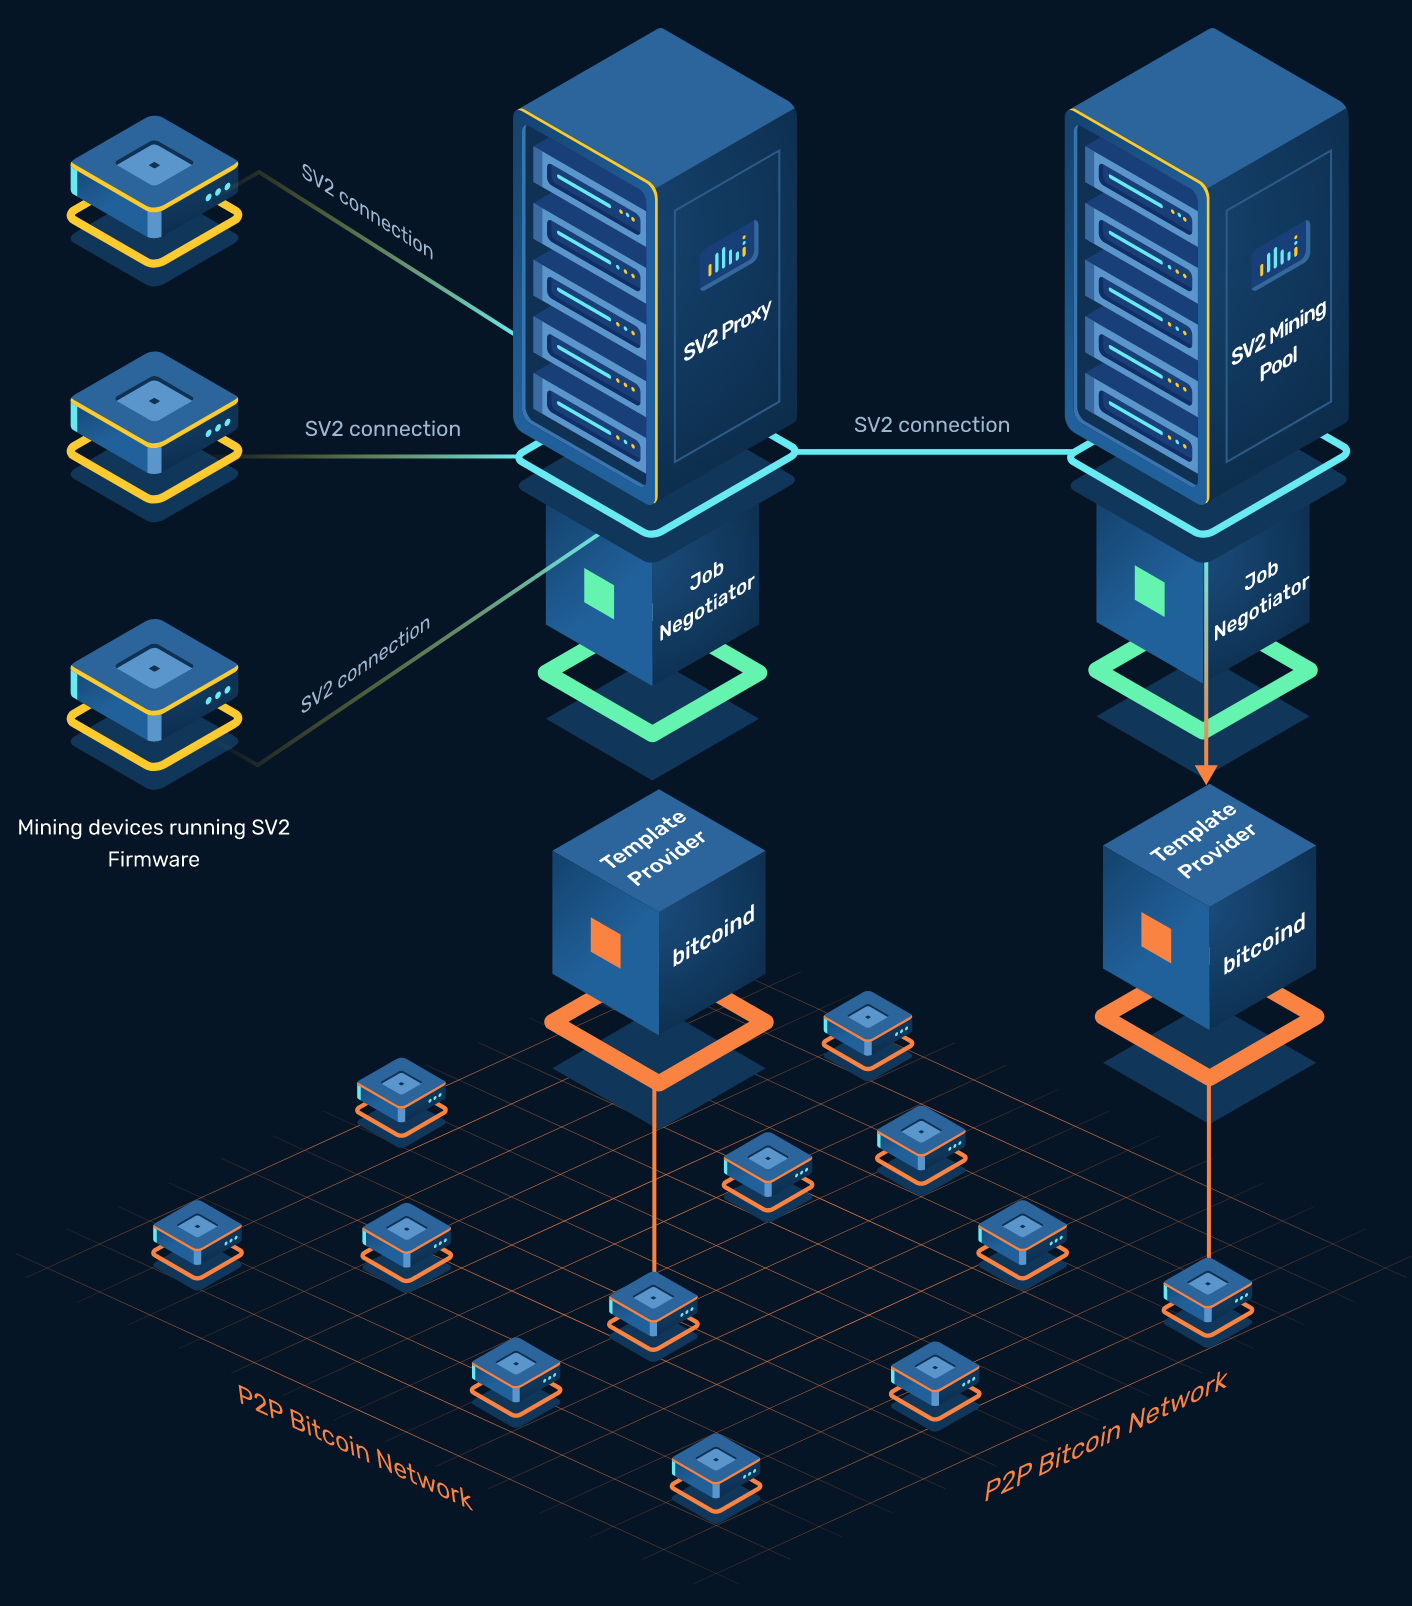
\includegraphics[width=8.5cm]{Figures/sri/SRI_configA.png}
    \captionof{figure}{SRI configuration A}
    \end{minipage}

    \begin{minipage}{.40\textwidth}
    \item \textbf{Configuration B}\label{configB}\\
    Mining Devices run SV2 firmware, so they are able to connect to a SV2 Mining Proxy (typically through a standard channel). The proxy aggregates all the standard channels opened into just one open channel with the SV2 Pool (group channel or an extended channel). In this configuration, the Proxy doesn't have the Job Declarator setup, so it's unable to select transactions from its local Template Provider. Transactions selection is done by the SV2 Pool, as it was done in Stratum V1, but now it can benefit from all the security and performance features brought by SV2. 
    \end{minipage}
    \hspace{0.25cm}
    \begin{minipage}{.60\textwidth}
    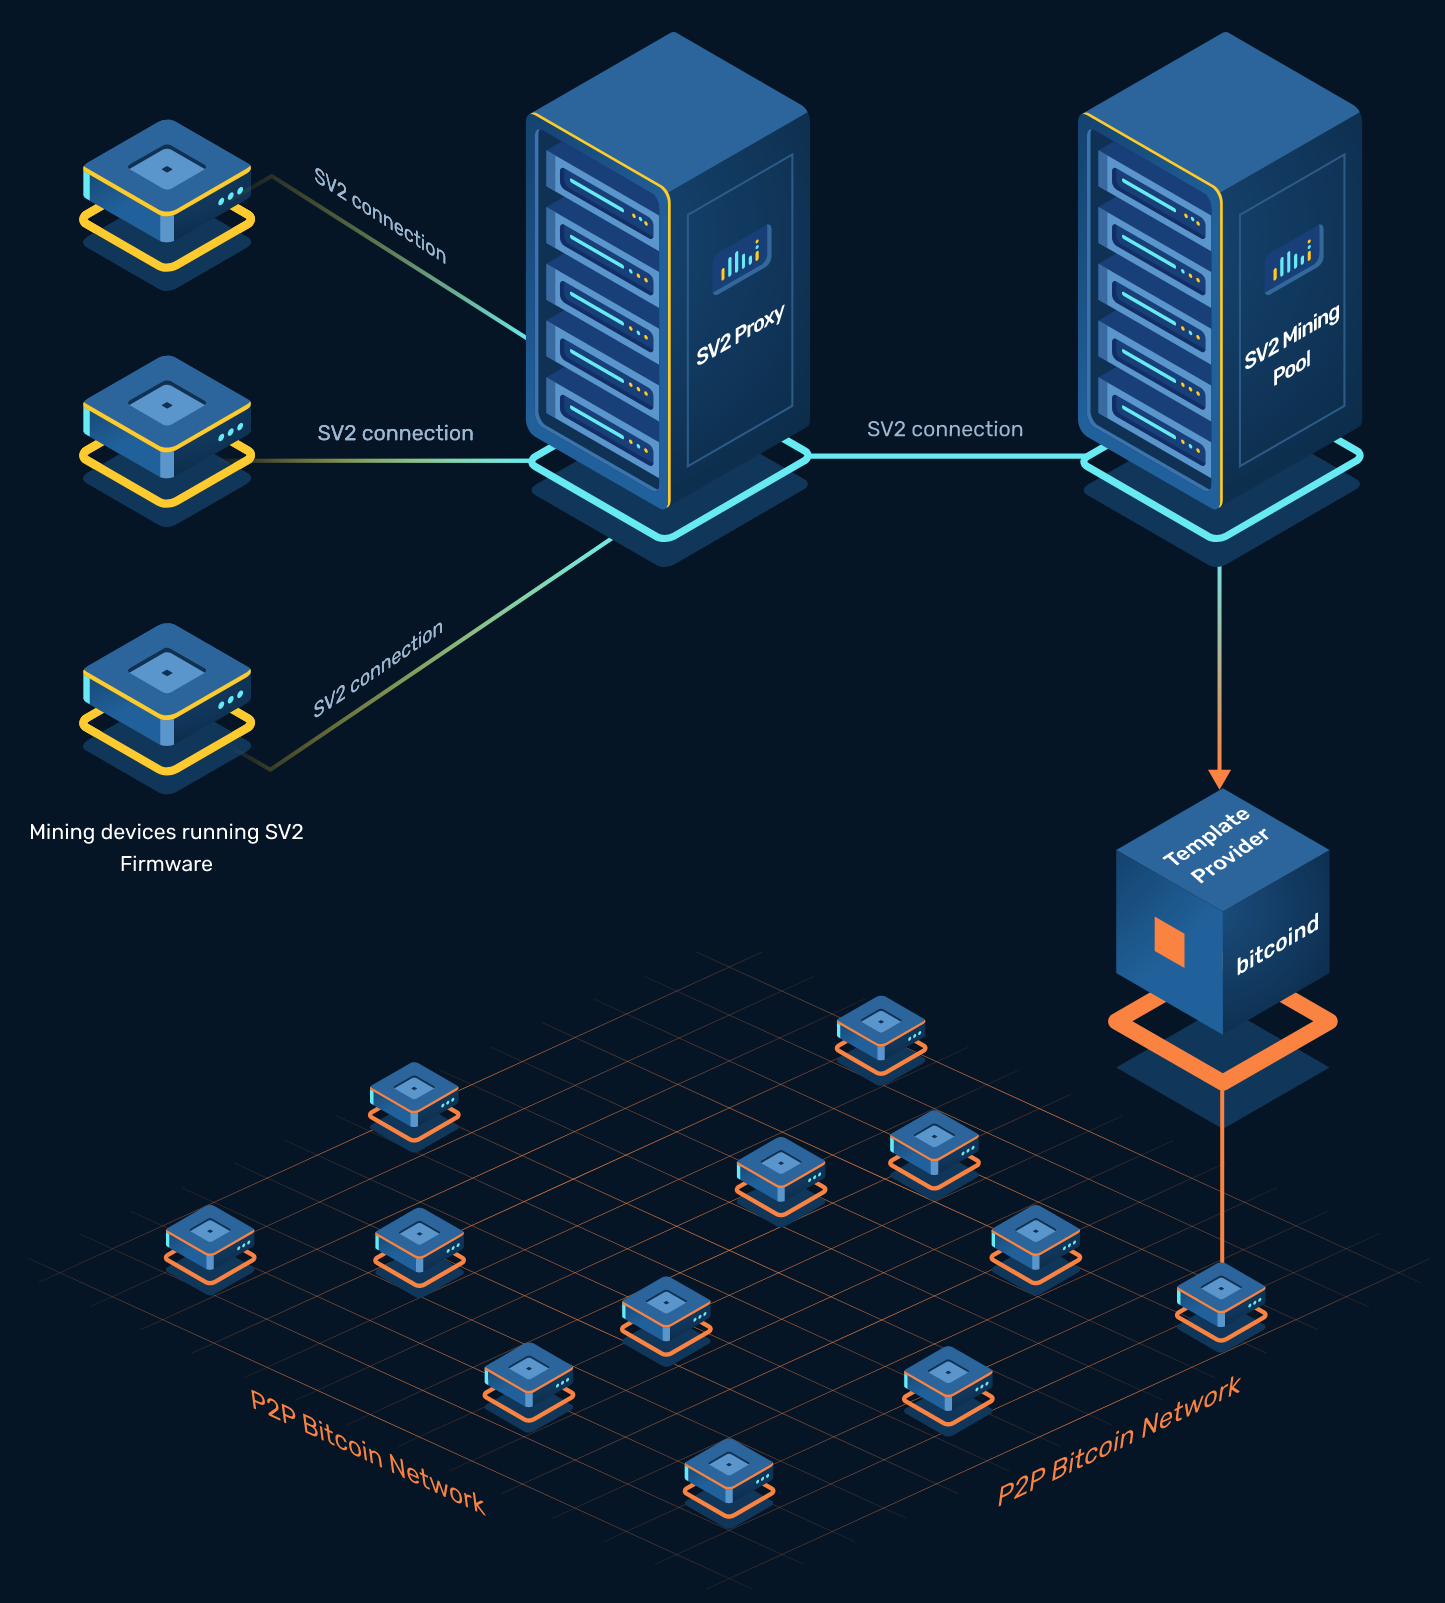
\includegraphics[width=8.5cm]{Figures/sri/SRI_configB.png}
    \captionof{figure}{SRI configuration B}
    \end{minipage}

    \begin{minipage}{.40\textwidth}
    \item \textbf{Configuration C}\label{configC}\\
    With this setup, Mining Devices don't need to run a SV2 compatible firmware. The Proxy which is used to let for efficiency, is also able to translate the SV1 messages that come from the Mining Device into SV2 messages for the SV2 Pool. In this case, the Translator Proxy is not configured to talk to a local Template Provider, so transactions selection is done by the pool. However, this configuration permits to test and use the SV2 protocol features without installing any other SV2 firmware on the machines.
    \end{minipage}
    \hspace{0.25cm}
    \begin{minipage}{.60\textwidth}
    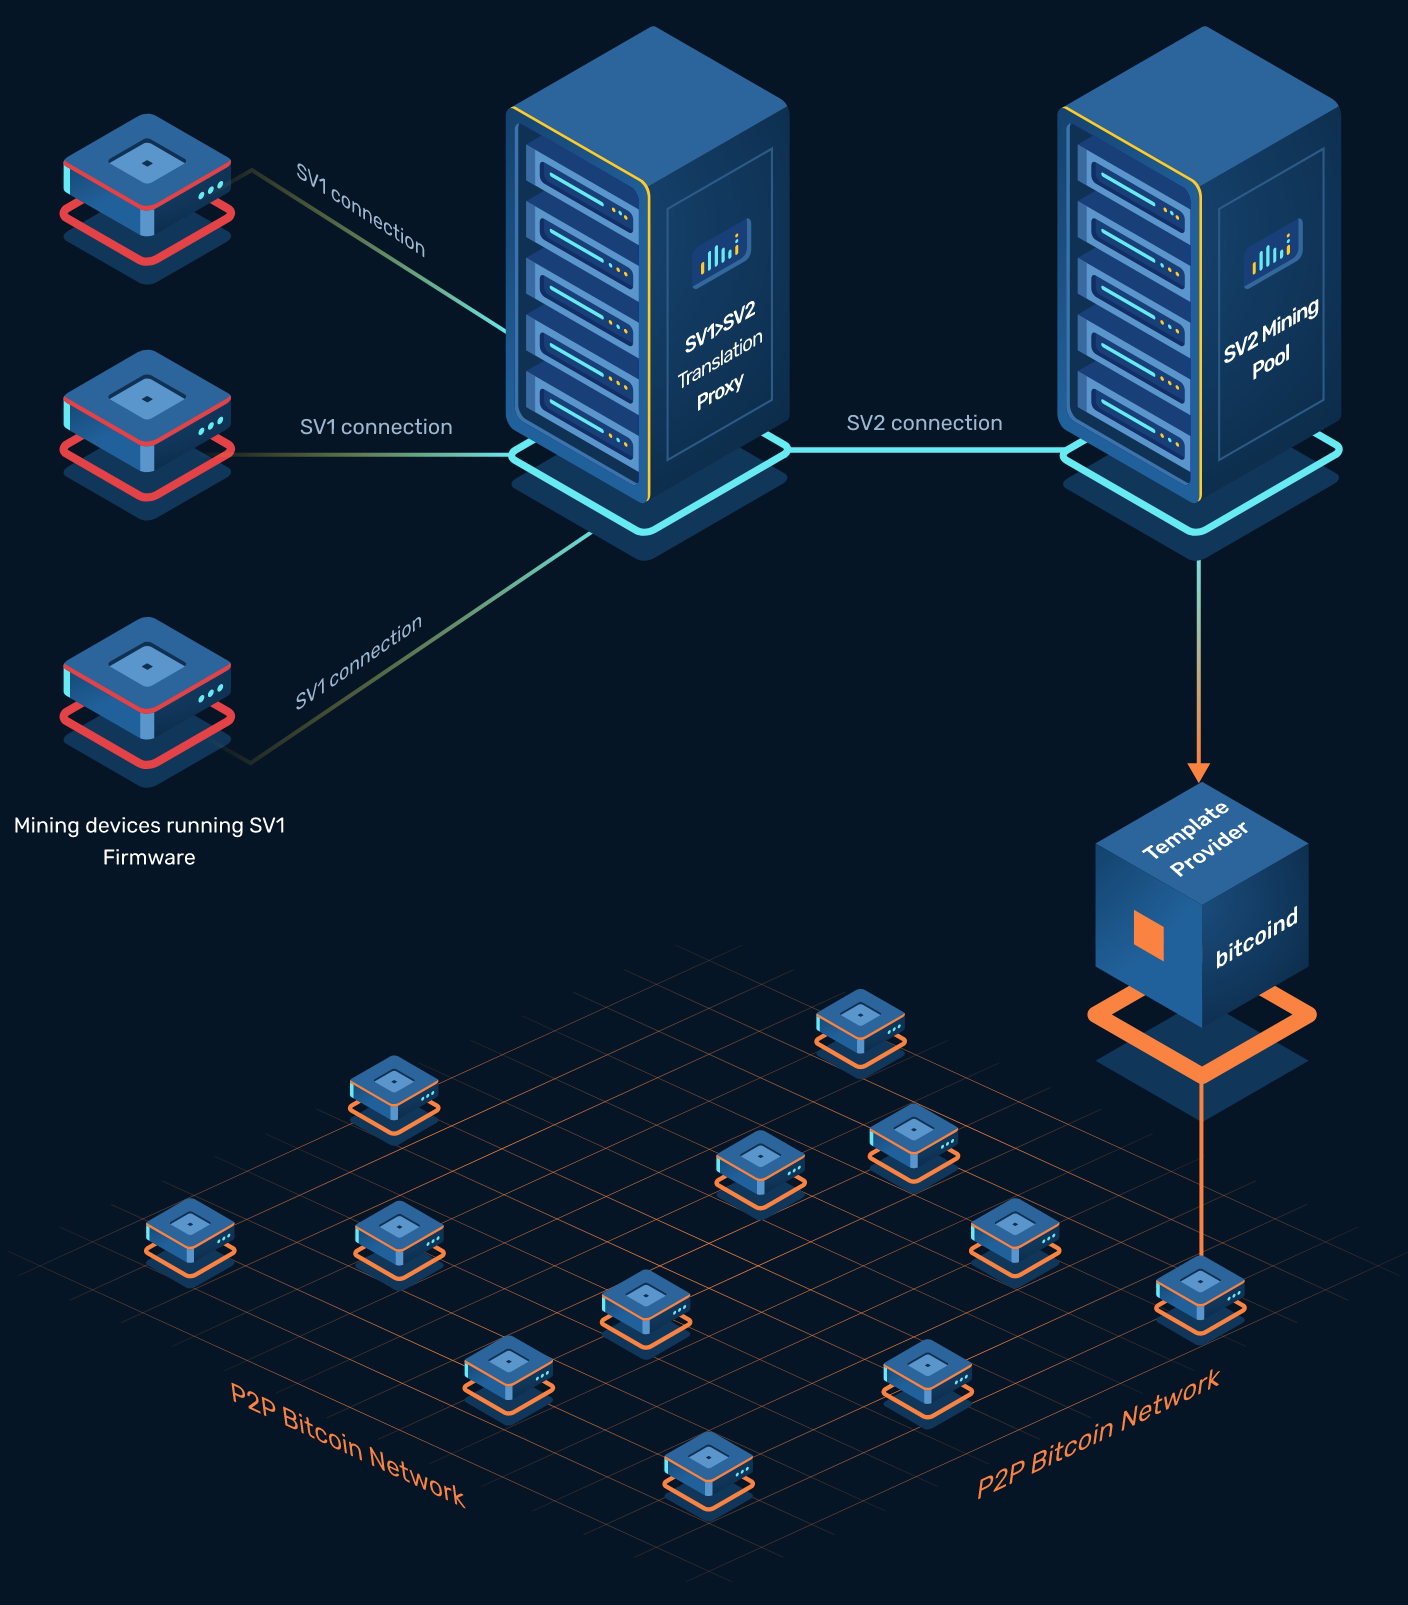
\includegraphics[width=8.5cm]{Figures/sri/SRI_configC.png}
    \captionof{figure}{SRI configuration C}
    \label{fig:SRI_configC}
    \end{minipage}

    \begin{minipage}{.40\textwidth}
    \item \textbf{Configuration D}\label{configD}\\
    This configuration is very similar to the previous (config C), but it's able to add the transactions selection feature to it. As represented in Figure \ref{fig:SRI_configD}, the Translator Proxy is joined by a Job Negotiator and a Template Provider: it's able, in this way, to build its own block templates and declare them to the SV2 Pool, through an extended channel.
    \end{minipage}
    \hspace{0.25cm}
    \begin{minipage}{.60\textwidth}
    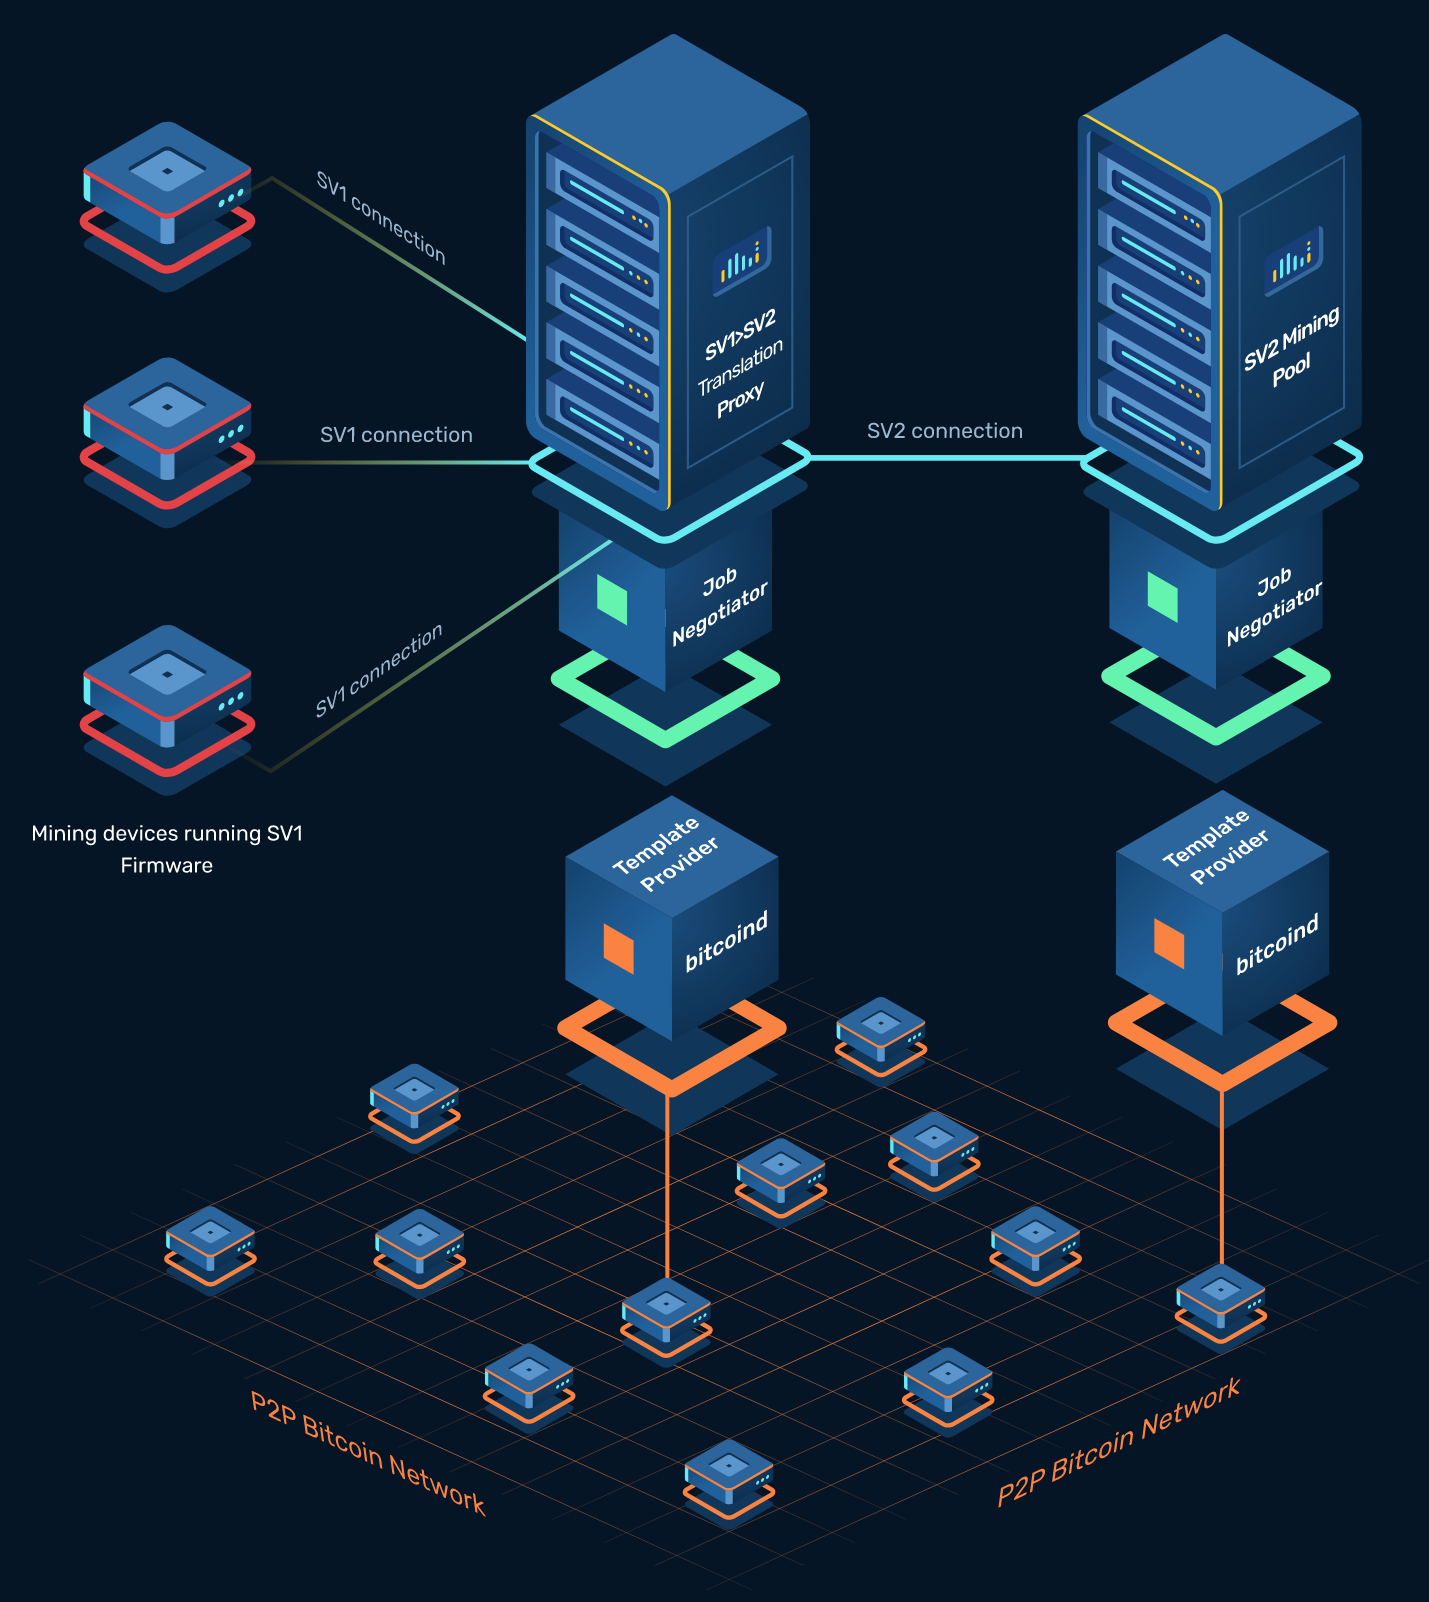
\includegraphics[width=8.5cm]{Figures/sri/SRI_configD.png} 
    \captionof{figure}{SRI configuration D}
    \label{fig:SRI_configD}
    \end{minipage}
    
\end{itemize}